\documentclass{article}

\usepackage{graphicx}
\usepackage{subfig}
\usepackage{float}
\usepackage{here}
\usepackage[T1]{fontenc} 
\usepackage{color}
\usepackage{multirow}
\usepackage{dblfloatfix} 

\usepackage{microtype}


% *** MATH PACKAGES ***
\usepackage[cmex10]{amsmath}
\usepackage{amssymb}
\usepackage{mathabx}
\usepackage{times}
\usepackage{bm}

% *** CITATION PACKAGES ***
%
\usepackage{cite}


% *** MATH PACKAGES ***
\usepackage[cmex10]{amsmath}
\usepackage{amssymb}
\usepackage{mathabx}
\usepackage{times}
\usepackage{bm}
\usepackage{accents}
%
\usepackage{algorithm}% http://ctan.org/pkg/algorithms
\usepackage{algpseudocode}% http://ctan.org/pkg/algorithmicx


\title{User Guide for MIDAS}
\author{Ines Fenni, Jet Propulsion Laboratory  \\
	Helene Roussel, Sorbonne University  \\
	}
\date{\today}
% Hint: \title{what ever}, \author{who care} and \date{when ever} could stand 
% before or after the \begin{document} command 
% BUT the \maketitle command MUST come AFTER the \begin{document} command! 
\begin{document}

\maketitle


\begin{abstract}
Short introduction to subject of the paper \ldots 
\end{abstract}

\section{Introduction}


\section{3D full wave model for scattering by complex-shaped objects}\label{3D_full_wave_model}
In order to rigorously compute the scattering properties of complex snow scatterer, we develop a 3D full-wave model based on the volumetric integral representation of the electric field, and we apply it to complex-shaped scatterer.

\subsection{Modeling of the electric field inside the scatterer based on the volumetric integral formulation} \label{VIEM-MoM}

\subsubsection{Volume Integral Equation Method (VIEM)}
The model developped to calculate the total field inside complex-shaped hydrometeors is based on the use of the volume integral equation method (VIEM) \cite{Nguyen2006model,Bellez2009model}, where the electric field $\vec{\textbf{E}}(\vec{\textbf{r}})$ at any point $\vec{\textbf{r}}$ inside the scatterer is given by 

%
\begin{equation}
\label{EQ_VIEM}
\vec{\textbf{E}}(\vec{\textbf{r}})= \vec{\textbf{E}}^i(\vec{\textbf{r}}) + (k_0^2 + \mathcal{r}\mathcal{r}.) \mathrm{\int_{\Omega}} \chi(\vec{\textbf{r}'})\text{ } \bar{\bar{\textbf{G}}}(\vec{\textbf{r}},\vec{\textbf{r}'})\text{ }\vec{\textbf{E}}(\vec{\textbf{r}'})d\vec{\textbf{r}'}
\end{equation}
%
where $\vec{\textbf{E}}(\vec{\textbf{r}})$ is the field inside the scatterer, $\vec{\textbf{E}}^i(\vec{\textbf{r}})$ is the incident field, $k_0$ is the wavelength number in the air, $\Omega$ represents the domain occupied by the scatterer, $\chi(\vec{\textbf{r}'})$ is the dielectric contrast at the location $\vec{\textbf{r}'}$ and $\bar{\bar{\textbf{G}}}(\vec{\textbf{r}},\vec{\textbf{r}'})$ is the free space dyadic Green's function.

In electromagnetic theory, the dyadic Green's function $\bar{\bar{\textbf{G}}}(\vec{\textbf{r}},\vec{\textbf{r}'})$ is essentially defined by the scattered
field  $\vec{\textbf{E}}$ at any observation point $\vec{\textbf{r}'}$ generated by a radiating electric dipole $\vec{\textbf{p}}$ located at the source position $\vec{\textbf{r}'}$. In mathematical terms this reads as 

\begin{equation}
\label{EQ_Green1}
\vec{\textbf{E}}(\vec{\textbf{r}})= \omega^2 \mu_0 \mu \bar{\bar{\textbf{G}}}(\vec{\textbf{r}},\vec{\textbf{r}'}) \vec{\textbf{p}} (\vec{\textbf{r}'})
\end{equation}

It verifies the equation 

\begin{equation}
\label{EQ_Green2}
(\mathcal{r}^2 + k_0^2) \bar{\bar{\textbf{G}}}(\vec{\textbf{r}},\vec{\textbf{r}'})  = - \delta (\vec{\textbf{r}}-\vec{\textbf{r}'}) \underline{I}
\end{equation}

where $\delta$ is the Dirac delta function and $\underline{I}$ is the identity. The dyadic green's function in free space is expressed as 

\begin{equation}
\label{EQ_Green3a}
\bar{\bar{\textbf{G}}}(\vec{\textbf{r}},\vec{\textbf{r}'}) = 
\begin{bmatrix}
G_{xx} & 0 & 0\\
0 & G_{yy} & 0\\
0 & 0 & G_{zz}
\end{bmatrix}
\end{equation}

\begin{equation}
\label{EQ_Green3b}
\textbf{G}_{pq}(\vec{\textbf{r}},\vec{\textbf{r}'}) = \dfrac{e^{jk_0|\vec{\textbf{r}}-\vec{\textbf{r}'}|}}{4\pi|\vec{\textbf{r}}-\vec{\textbf{r}'}|}
\end{equation}

where $p,q = x,y,z$. It is worth noting that the dyadic green's function in free space is expressed in the spectral domain as  

\begin{equation}
\label{EQ_Green4a}
\bar{\bar{\textbf{G}}}(\vec{\textbf{r}},\vec{\textbf{r}'}) = \int\int_{-\infty}^{+\infty} g^s_{pq}(\nu,\eta,z,z')e^{j2\pi[\nu(x-x')+\eta(y-y')]}d\nu d\eta
\end{equation}

\begin{equation}
\label{EQ_Green4b}
g^s_{pq}(\nu,\eta,z,z') = \dfrac{j}{2\gamma_0}e^{j\gamma_0|z-z'|}
\end{equation}
where $p,q = x,y,z$,  $\gamma_0 = \sqrt{k_0^2-4\pi^2(\nu^2+\eta^2)}$, $\nu=\dfrac{k_{0x}}{2\pi}$, , $\eta=\dfrac{k_{0y}}{2\pi}$, and $k_{0x}$ and $k_{0y}$ are the components of the free space wave vector $k_0$ along $x$ and $y$, respectively. 

\subsubsection{Calculation of the Incident Field $\vec{\textbf{E}}^i(\vec{\textbf{r}})$} 
We consider an incident plane wave propagating along $\hat{k}_i = \dfrac{\vec{\textbf{k}}_i}{k_0}$, polarized vertically or horizontally, depending if $\hat{e}_i=\hat{v}_i$ or $\hat{e}_i=\hat{h}_i$, respectively, as described in "here reference to Bringi". $\hat{k}_i$ is set by the angles $\theta_i$ and $\phi_i$ where, depending on the used convention (DDScat- or ADDA-equivalent respectively), $\theta_i$ describes the rotation around $\hat{z}$ or $\hat{y}$, and $\phi_i$ describes the rotation around $\hat{x}$ or $\hat{z}$. (see figures - Not included yet for ADDA convention). Knowing that any observation point is described in the Cartesian reference as $\vec{\textbf{r}}=x\hat{x}+y\hat{y}+z\hat{z}$, the incident electric field, $\vec{\textbf{E}}^i(\vec{\textbf{r}})$, is expressed at any observation point $\vec{\textbf{r}}$ as

\begin{equation}
\label{EQ_Einc}
\vec{\textbf{E}}^i(\vec{\textbf{r}}) = \hat{e}_i E_0 e^{jk_0\hat{k}_i\vec{\textbf{r}}}
\end{equation} 

Depending on the used convention, DDScat- (Eq. \ref{EQ_Einc_DDScat}) or ADDA- (Eq. \ref{EQ_Einc_ADDA}), the wave and polarization unit vectors ($\hat{k}_i$, $\hat{v}_i$, $\hat{h}_i$) are expressed as 

\begin{equation}
\label{EQ_Einc_DDScat}
\begin{bmatrix}
\hat{k}_i \\
\hat{v}_i \\
\hat{h}_i 
\end{bmatrix} = 
\begin{bmatrix}
\cos(\theta_i) & \sin(\theta_i)*\cos(\phi_i) & \sin(\theta_i)*\sin(\phi_i)\\
- \sin(\theta_i) & \cos(\theta_i)*\cos(\phi_i) & \cos(\theta_i)*\sin(\phi_i)\\
0 & - \sin(\phi_i) & \cos(\phi_i)\\
\end{bmatrix}
\begin{bmatrix}
\hat{x} \\
\hat{y} \\
\hat{z} 
\end{bmatrix}
\end{equation}     

\begin{figure}[H]
	\centering
	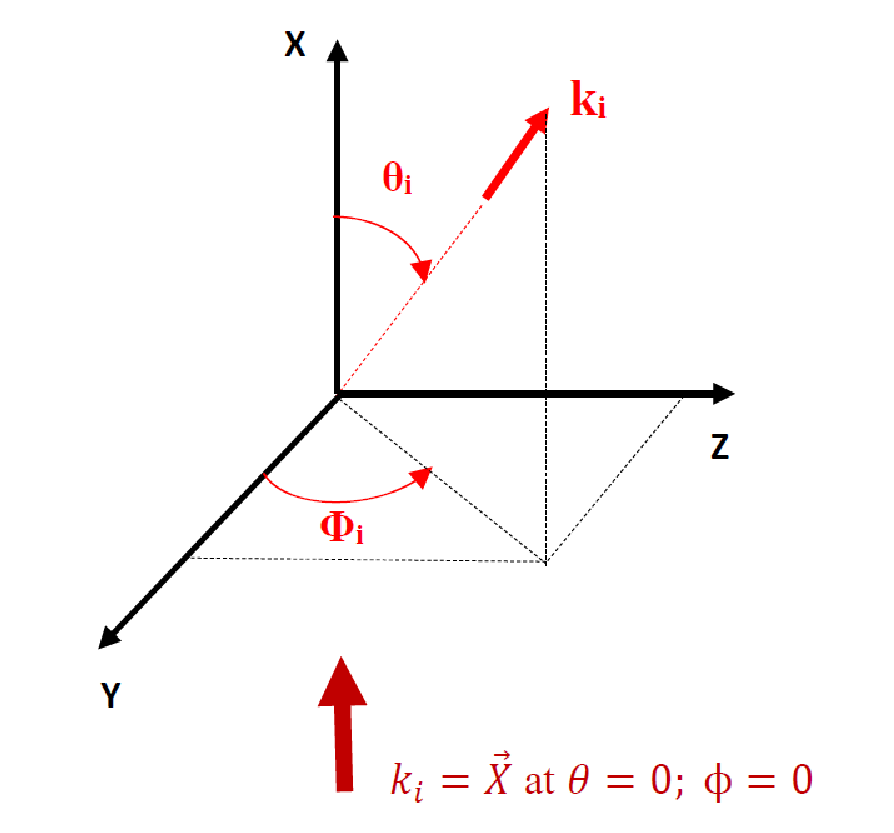
\includegraphics[scale=0.5]{Figures/Einc_figure1.eps}
	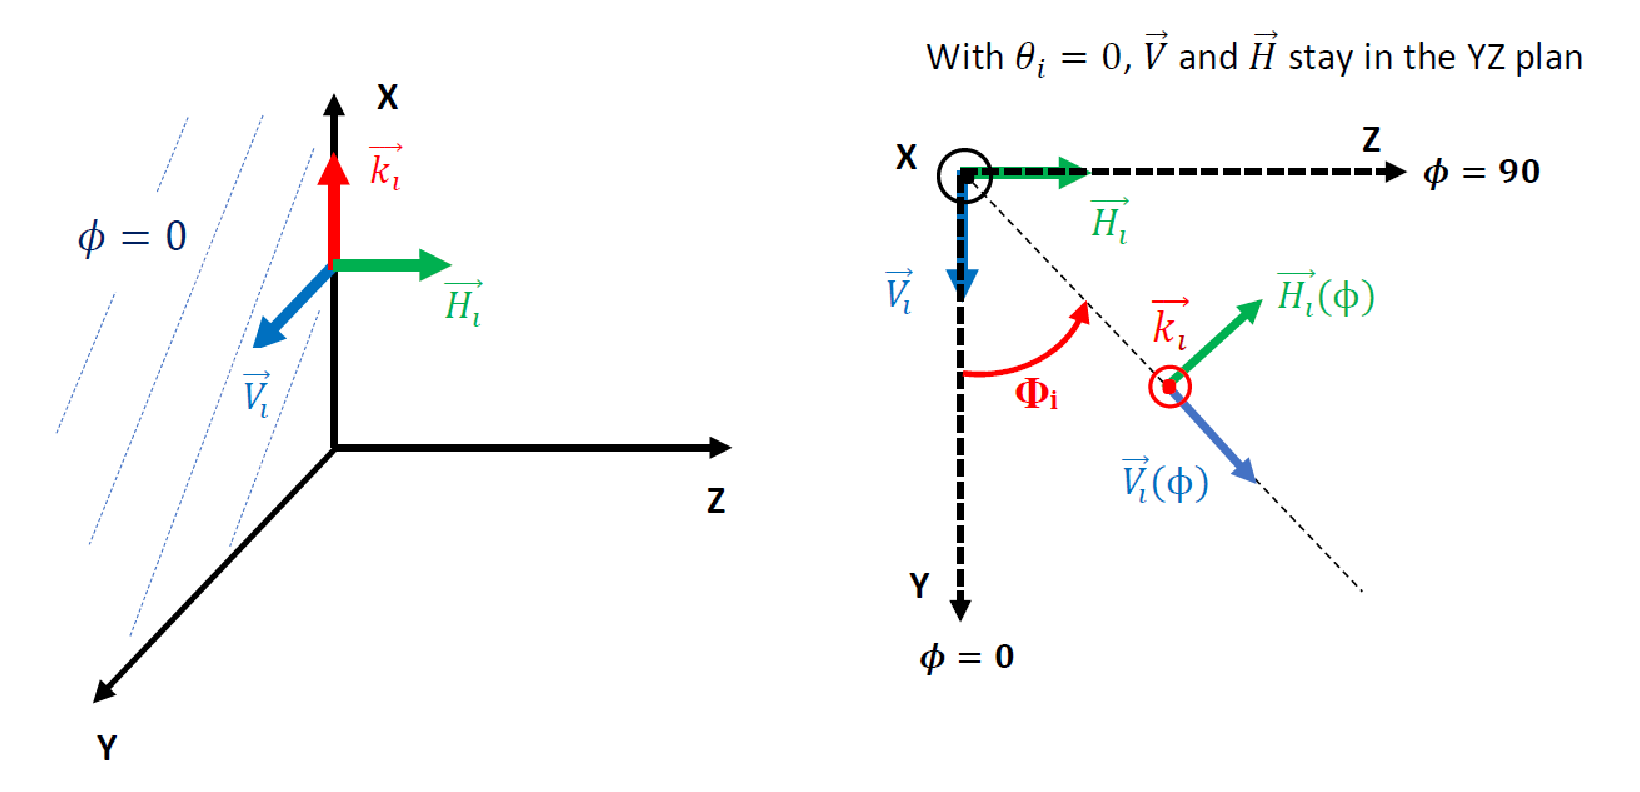
\includegraphics[scale=0.5]{Figures/Einc_figure2.eps}
	\caption{Incident EM wave direction in DDScat convention (Eq. \ref{EQ_Einc_DDScat}).}
	\label{Fig_Einc}
\end{figure} 

\begin{equation}
\label{EQ_Einc_ADDA}
\begin{bmatrix}
\hat{k}_i \\
\hat{v}_i \\
\hat{h}_i 
\end{bmatrix} = 
\begin{bmatrix}
\sin(\theta_i)*\cos(\phi_i) & \sin(\theta_i)*\sin(\phi_i) & \cos(\theta_i) \\
\cos(\theta_i)*\cos(\phi_i) & \cos(\theta_i)*\sin(\phi_i) & - \sin(\theta_i)\\
- \sin(\phi_i) & \cos(\phi_i) & 0\\
\end{bmatrix}
\begin{bmatrix}
\hat{x} \\
\hat{y} \\
\hat{z} 
\end{bmatrix}
\end{equation}     

\subsubsection{The Method of Moments} 

Next, the volumetric integral equation is solved by means of a Method of Moments (MoM). To do so, Eq. \ref{EQ_VIEM} is rewritten as       

\begin{equation}
\label{EQ_VIEM_re_1}
\bar{\bar{\Gamma}} \vec{\textbf{E}}(\vec{\textbf{r}})= \vec{\textbf{E}}^i(\vec{\textbf{r}}) 
\end{equation}
\begin{equation}
\label{EQ_VIEM_re_2}
\text{where	} \bar{\bar{\Gamma}} = \bar{\bar{\textbf{I}}} - (k_0^2+\mathcal{r}\mathcal{r}.) \mathrm{\int_{\Omega}} \chi(\vec{\textbf{r}'})\text{ }\bar{\bar{\textbf{G}}}(\vec{\textbf{r}},\vec{\textbf{r}'})\text{ }d\vec{\textbf{r}'} \nonumber
\end{equation}

 The MoM begins with the discretization of object into $N$ cubic cells $\Omega_n$, of side $S_c$, which is small enough to enable us to assume that the electric field inside is constant. To meet this requirement, and thus to ensure the accuracy of the MoM solution, the cell size should be equal to or lower than $\lambda_s/10$, with $\lambda_s=\lambda_0/\sqrt{\epsilon_r}$. $\lambda_s$ is the wavelength inside the scatterer, $\lambda_0$ is the free space wavelength and $\epsilon_r$ is the real part of the relative permittivity of the discretized domain. 
 Fig. \ref{Fig_MoM_discretization} shows an example of discretization of a simple spherical particle and of 3 typical snow crystals : a star-shaped dendrite, a dendrite with broadening arms and a sandwich plate.
 \begin{figure}[H]
 	\centering
 	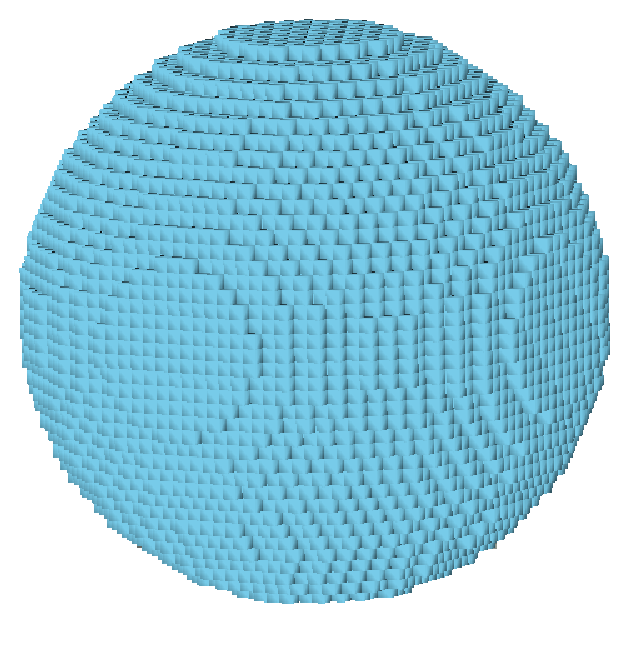
\includegraphics[scale=0.3]{Figures/discretizationSphere.eps}
 	\hspace{0.5cm}
 	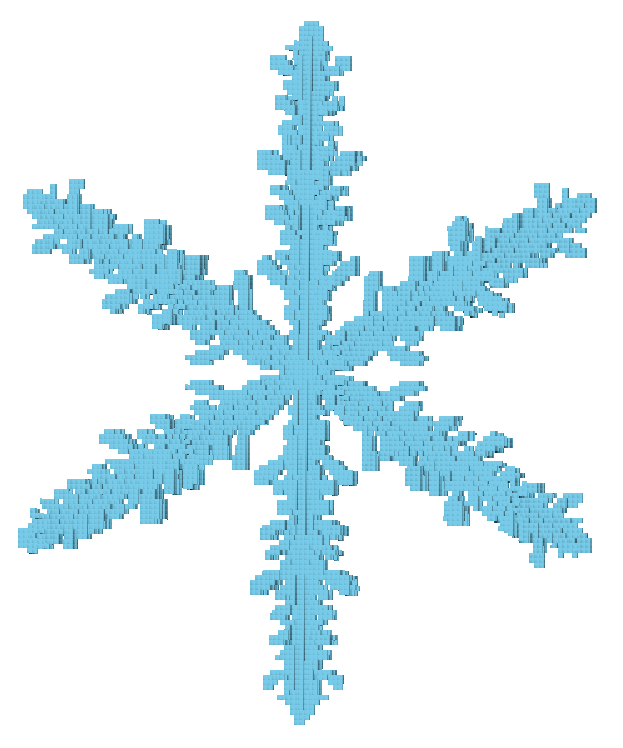
\includegraphics[scale=0.3]{Figures/discretization_p13.eps}
 	\hspace{0.5cm}
 	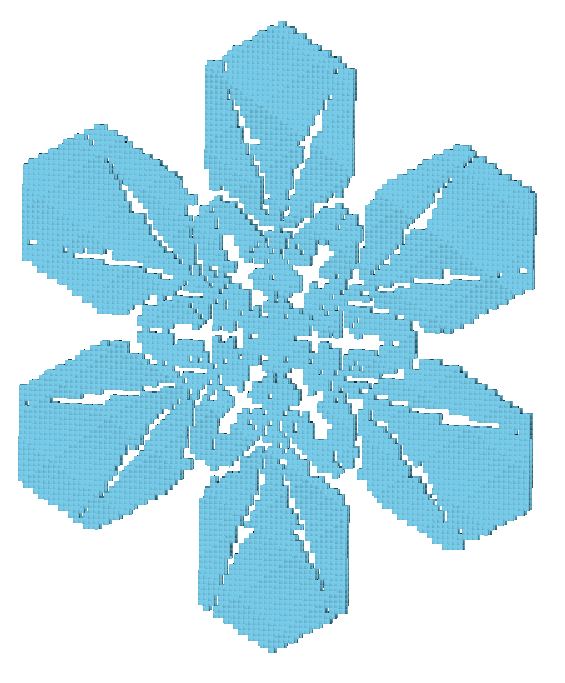
\includegraphics[scale=0.3]{Figures/discretization_p46.eps}
 	\caption{Examples of discretization into cubic cells (or voxels).}
 	\label{Fig_MoM_discretization}
 \end{figure} 

After discretization into $N$ cells, the field inside the scatterer is decomposed as

\begin{equation}
\label{EQ_MoM1}
\vec{\textbf{E}}(\vec{\textbf{r}}) = \sum_{n=1}^{N}\sum_{q=1}^3 E_q^n \bar{\textbf{F}}_q^n(\vec{\textbf{r}})
\end{equation} 

where $E_q^n$ is the constant unknown of $\bar{\textbf{F}}_q^n$, the $n^{th}$ basis function for the component ($q=x$, $y$ or $z$) of the field inside the scatterer. To select a set of test functions $W_p^m$ ($m=1$,..,$M$ and $p=x$, $y$, $z$), the point matching method is used. So, $M=N$ and $\bar{\textbf{W}}_p^m$ is a Dirac delta function located at the center of the cell $\Omega_n$. Eq. \ref{EQ_VIEM_re_1} is re-written : 

\begin{equation}
\label{EQ_MoM2-a}
\sum_{n=1}^{N}\sum_{q=1}^3 \Big \langle \bar{\textbf{W}}_p^m, \bar{\bar{\Gamma}} \bar{\textbf{F}}_q^n \Big \rangle E^n_q = \Big \langle \bar{\textbf{W}}_p^m, \bar{\textbf{E}}^i \Big \rangle
\end{equation}  
\begin{equation}
\label{EQ_MoM2-b}
\text{Where } \bar{\textbf{F}}_q^n(\vec{\textbf{r}}) = 
\begin{Bmatrix}
1; & \vec{\textbf{r}} \in \Omega_n\\
0; & \vec{\textbf{r}} \notin \Omega_n
\end{Bmatrix}
\: \hat{q} 
\nonumber
\end{equation}

 
\begin{equation}
\label{EQ_MoM2-c}
\text{ and } \bar{\textbf{W}}_p^m(\vec{\textbf{r}}) = \delta(\vec{\textbf{r}}-\vec{\textbf{r}}_m) \: \hat{p} 
\nonumber
\end{equation} 

This results in the system of $N$ linear equations    
\begin{equation}
\label{EQ_MoM3-a}
\sum_{n=1}^{N}\sum_{q=1}^3 \textbf{Z}_{pq}^{mn} \textbf{E}_q^n = \textbf{E}_p^{i,m}
\end{equation} 
that we can simply express as   
\begin{equation}
\label{EQ_MoM3-b}
\textbf{Z} \textbf{E} = \textbf{E}^i
\end{equation} 

where \textbf{Z} is the $3N \times 3N$ full matrix representing the interactions between the cells composing the scatterer, $\textbf{E}^i$ is the incident field of size $3N$ and $\textbf{E}$ is the unknown solution vector of size $3N$ that represents the total electric field inside the scatterer in the $q$ (=$x$, $y$ or $z$) direction.

The elements of $\textbf{Z} = \left[ Z_{pq}^{mn} \right]$ are given by $Z_{pq}^{mn} = \delta_{mn} \delta{pq} - Z_{pq}^{f, mn}$ where 

\begin{equation}
\label{EQ_MoM4}
Z_{pq}^{f, mn} = k_0^2 \int_{\Omega_n} \chi(\vec{\textbf{r}}'_n) G_{pq}^f(\vec{\textbf{r}}_m,\vec{\textbf{r}}'_n) d\vec{\textbf{r}}'_n + \sum_{q=1}^{3} \dfrac{\partial^2}{\partial p_m \partial q_m} \int_{\Omega_n} \chi(\vec{\textbf{r}}'_n) G_{pq}^f(\vec{\textbf{r}}_m,\vec{\textbf{r}}'_n) d\vec{\textbf{r}}'_n
\end{equation} 

where $\vec{\textbf{r}}_m$ points to the observation point $m$, and $\vec{\textbf{r}}'_n$ points to the center of the source cell $n$, $G_{pq}^f$ is the component $pq$ of the dyadic Greens function given by Eq. \ref{EQ_Green3b}, and $\chi(\vec{\textbf{r}}') = \dfrac{\epsilon(\vec{\textbf{r}}')-\epsilon_0}{\epsilon_0}$ is the dielectric contrast. Given that the domain $\Omega_n$ is homogeneous, $\chi(\vec{\textbf{r}}')$ does not depend on the position $\vec{\textbf{r}}'$. We can then write :

\begin{equation}
\label{EQ_MoM_Chi1}
\int_{\Omega_n} \chi(\vec{\textbf{r}}'_n) G_{pq}^f(\vec{\textbf{r}}_m,\vec{\textbf{r}}'_n) d\vec{\textbf{r}}'_n = \chi_n \int_{\Omega_n} G_{pq}^f(\vec{\textbf{r}}_m,\vec{\textbf{r}}'_n) d\vec{\textbf{r}}'_n
\end{equation} 
\begin{equation}
\label{EQ_MoM_Chi2}
\text{where} \; \;  \chi_n = \epsilon_{r,n} - 1 \nonumber
\end{equation}    

If $m=n$, in order to avoid singularities, $Z_{pq}^{f,mn}$ is computed using Hadamard regularization. The integral on $\Omega_n$ is approximated by an integral on sphere of radius 

\begin{equation}
\label{EQ_MOM_an}
a_n=S_c\sqrt[3]{3/(4\pi)}
\end{equation} 

So, we obtain the following 

\begin{equation}
\label{EQ_MoM_m-eq-n}
\begin{aligned}
\text{If } m=n \text{ : } Z_{pq}^{f, mn} & = \mathcal{H} \bigg ( \int_{\Omega_n} (k_0^2+\dfrac{\partial^2}{\partial p_m^2})G^f_{pq} (\vec{\textbf{r}}_m,\vec{\textbf{r}}'_n) d\vec{\textbf{r}}'_n \bigg )  \chi_n \\
& = \bigg ( \dfrac{2}{3} \; e^{jk_0a_n}(1-jk_0a_n) - 1 \bigg )  \chi_n  & \text{ if } p=q \\
Z_{pq}^{f, mn} & = 0 &\text{ if } p \ne q 
\end{aligned}
\end{equation} 

With $m \ne n$, we can integrate numerically the elements of the dyadic Green's function over the domain $\Omega_n$. But, this will result in a  computational cost. So, we have chosen to approximate the integration of $G_{pq}^f(\vec{\textbf{r}}_m,\vec{\textbf{r}}'_n)$ over a cubical cell of side size $S_c$ by an integration over a sphere of equivalent radius $a_n$ (Eq. \ref{EQ_MOM_an}) as follows

\begin{equation}
\label{EQ_MoM-m-neq-n_1}
\int_{\Omega_n} G^f_{pq} (\vec{\textbf{r}}_m,\vec{\textbf{r}}'_n) d\vec{\textbf{r}}'_n = \kappa_n \; G^f_{pq} (\vec{\textbf{r}}_m,\vec{\textbf{r}}'_n)
\end{equation} 
\begin{equation}
\label{EQ_MoM-m-neq-n_2}
\text{where } \; \; \kappa_n = 4\pi \dfrac{sin(k_0a_n)-k_0a_ncos(k_0a_n)}{k_0^3}  \nonumber
\end{equation} 

Thus, the elements of $Z_{pq}^{f, mn}$, with $m \ne n$, are computed as follows  

\begin{equation}
\label{EQ_MoM_Zmnpq}
Z_{pq}^{f, mn} = 
\left \lbrace
\begin{array}{l l}
\dfrac{e^{j k_0 r_{mn}}}{4 \pi r^2_{mn}} \; \big ( \tau_{mn} + k^2_0 \big (r_{mn} - \dfrac{(p_m-q_n')^2}{r_{mn}} \big ) - 3 \dfrac{(p_m-q_n')^2}{r^2_{mn}} \tau_{mn} \big ), & m \ne q, \; p=q \\
\text{ } & \text{ } \\
\dfrac{e^{j k_0 r_{mn}} (p_m-p'_n) (q_m-q'_n)}{4 \pi r_{mn}^3} \; (-k_0^2 - \dfrac{3}{r_{mn}} \tau_{mn}) \kappa_n, & m \ne q, \; p \ne q
\end{array} \right . 
\end{equation}
where $\tau_{mn} = jk_0 - \dfrac{1}{r_{mn}}$, and $r_{mn} = \sqrt{(x_m-x'_n)^2 + (y_m-y'_n)^2 + (z_m-z'_n)^2}$ is the distance between the center of the observation cell $m$ and the center of the source cell $n$.

Further details about the free space Green's function, the selection of basis and test functions and the calculation of the MoM matrix elements are available in \cite{Nguyen2006model,Bellez2009model}.
Since our 3D full-wave model is based on the use of piecewise constant basis functions with the VIEM, it is mathematically close to the DDA \cite{penttila2007comparison}.     

To summarize, an application of a conventional MoM to a complex-shaped scatterer discretized into $N_c$ cubic cells results in a system of linear equations corresponding to a full matrix $\textbf{Z}^{MoM}$ of size $3N_c\times3N_c$. Therefore, with a complexity of $O(N^3)$ in time and of $O(N^2)$ in storage, where $N=3N_c$,  the model is so computationally extensive that it becomes very quickly untenable as we increase $N$. That is exactly the type of scenario where the CBFM is well suited to solve the problem at hand in an efficient manner. 



\subsection{Calculated scattering quantities} \label{Scattering_Quantities}
Once $\vec{\textbf{E}}(\vec{\textbf{r}})$ the total electric field inside the object is known, $\vec{\textbf{E}}^s(\vec{\textbf{r}})$ the scattered field at any point $\vec{\textbf{r}}$ is given by    

\begin{equation}
\label{EQ_VIEM_scat}
\vec{\textbf{E}}^s(\vec{\textbf{r}})= (k_0^2 + \mathcal{r}\mathcal{r}.) \mathrm{\int_{\Omega}} \chi(\vec{\textbf{r}'})\text{ }\bar{\bar{\textbf{G}}}(\vec{\textbf{r}},\vec{\textbf{r}'})\text{ }\vec{\textbf{E}}(\vec{\textbf{r}'}) \text{ }d\vec{\textbf{r}'}
\end{equation}

Example : 


Similarly to the calculation of the electric field inside the scatterer, the discretization of this integral equation leads to the following matrix system 

\begin{gather}
	\label{EQ_VIEM_scat_matrix}
	[\textbf{D}_{pq}^{s,n}][\textbf{E}_q^{n,i}] = [\textbf{E}_q^{s\textbf{ } n,i}] \\  
	\text{ with } q=[x,y,z]\text{; } n=1,..,N_c \nonumber \\
	i=1,..,N_{inc}\text{ and } s=1,..,:N_{sca} \nonumber
\end{gather}
where $\textbf{D}$ is a $3N_{sca} \times 3N_c$ matrix representing the $3$ components $x$, $y$ and $z$ of the scattered field from each cell $n \leq Nbc$ in the observation point $1 \leq s \leq N_{sca}$, $\textbf{E}$ of size $3Nbc \times N_{inc}$ is the total electric field inside the scatterer calculated for each incident EM wave $1 \leq i \leq N_{inc}$, and $\textbf{E}^s$ of size $N_{sca} \times N_{inc}$ represents the scattered field obtained at the observation points $s$ with the incident EM waves $i$. Therefore, once the electric field inside the scatterer is known for the $N_{inc}$ incident directions, the calculation of the scattered field at the $N_{sca}$ observation points scales as $O(N_c  N_{inc}N_{sca})$. Note also that the calculation of $\textbf{E}^s$ is embarrassingly parallel and so can be easily accelerated by the use of a large number of MPI processes. 

Next, the scattering matrix $\textbf{S}$ for each incident direction is derived from the scattered fields \cite{mishchenko2002scattering}, and the extinction, scattering and back-scattering efficiency factors $Q_{ext} = C_{ext}/\pi a^2$, $Q_{scat}=C_{scat}/\pi a^2$ and $Q_{bks}=C_{bks} /\pi a^2$ are calculated. $C_{ext}$, $C_{scat}$ and $C_{bks}$ are the scattering cross-sections and $a$ represents the effective radius of a particle of volume $V$, which is defined by $a = (3V/4\pi)^{1/3} = (3N_c/4\pi)^{1/3}S_c$ where $S_c$ is the size of cell used to discretize the particle. For each incident direction defined by ($\theta_i$, $\Phi_i$), $C_{ext}$, $C_{scat}$ and $C_{bks}$ are derived from the scattering matrix $S$ as follows \cite{mishchenko2002scattering}

\begin{gather}
	C_{ext} = \dfrac{2\pi}{k} [\Im\{\textbf{S}_{VV}(\theta_{fwd},\Phi_{fwd})\} + \Im\{\textbf{S}_{HH}(\theta_{fwd},\Phi_{fwd})\}] \\
	C_{scat} = \dfrac{1}{2k}\int_0^{2\pi}\int_0^{\pi}[\textbf{S}_{VV}(\theta_s,\Phi_s)^2+\textbf{S}_{VH}(\theta_s,\Phi_s)^2+ \nonumber\\
	\textbf{S}_{HV}(\theta_s,\Phi_s)^2+\textbf{S}_{HH}(\theta_s,\Phi_s)^2]\sin\theta \text{ } d\theta d\Phi \\
	C_{bks} = \dfrac{1}{2k} [\textbf{S}_{VV}(\theta_{bks},\Phi_{bks})^2+\textbf{S}_{VH}(\theta_{bks},\Phi_{bks})^2+ \nonumber 
	\\\textbf{S}_{HV}(\theta_{bks},\Phi_{bks})^2+\textbf{S}_{HH}(\theta_{bks},\Phi_{bks})^2]
\end{gather}
where ($\theta_s$, $\Phi_s$) describes the scattering direction, and ($\theta_{fwd}$, $\Phi_{fwd}$) and ($\theta_{bks}$, $\Phi_{bks}$) refers respectively to the scattering-forward and the backscattering directions.

Next, an averaging of the scattered properties is performed over the calculated incident directions defined by ($\theta_i$,$\phi_i$), as follows  
\begin{equation}
<Q> = \frac{1}{\Omega} \int_0^{\phi_{m}} \int_{0}^{\theta_{m}} Q(\theta, \phi) \sin\theta_i \text{ } d\theta_i \text{ } d\phi_i
\label{equ_AvScat}
\end{equation} 
where the choice of $0 \leq \phi_m \leq 2\pi$ and $0 \leq \theta_m \leq \pi$ strongly depends on the geometry of the snow particle, particularly on the symmetries that it presents. The solid angle $\Omega$ is calculated as $\int_0^{\phi_{m}} d\phi \int_{0}^{\theta_{m}} \sin\theta \text{ } d\theta$.
For the DDScat code, orientationally avearged scattering quantities are computed by evaluating them over a certain number of particle orientations. Thus, DDScat computes the orientational average $<Q>$ of a quantity $Q(\beta, \theta, \phi)$ \cite{draine2013user} as
\begin{equation}
<Q> = \frac{1}{8\pi^2} \int_0^{2\pi} d\beta \int_{-1}^1 d\cos\theta \int_0^{2\pi} d\phi \text{ } Q(\beta, \theta, \phi)
\label{equ1}
\end{equation} 
where the Euler angles ($\beta$, $\theta$ and $\phi$) are used to describe the 3D orientation of the snow particle. The DDScat code also enables the user to take advantage of the symmetries presented by the simulated particle by choosing the range of values of $\beta$, $\theta$ and $\phi$ \cite{draine2013user}. 
Since it is based on iterative solver, the computational cost for DDScat increases very rapidly with the number of target orientations, particularly in the case of electrically large particles. This is due to the recalculation of the entire EM problem for each target orientation. On the other hand, using a direct solver-based method, the NESCoP code is expected to largely outperform DDScat in terms of CPU time when computing orientationally averaged scattering by electrically large snow particles with a high number of incident directions (abbreviated as \textbf{id} for the MoM/CBFM code) or target orientations (abbreviated as \textbf{to} for DDSCat). 


%\begin{itemize}
%\item article
%\item book 
%\item report 
%\item letter 
%\end{itemize}
%
%
%\begin{enumerate}
%\item article
%\item book 
%\item report 
%\item letter 
%\end{enumerate}
%
%\begin{description}
%\item[article\label{article}]{Article is \ldots}
%\item[book\label{book}]{The book class \ldots}
%\item[report\label{report}]{Report gives you \ldots}
%\item[letter\label{letter}]{If you want to write a letter.}
%\end{description}


\section{Conclusions}\label{conclusions}
There is no longer \LaTeX{} example which was written by \cite{doe}.

\bibliographystyle{unsrt}
\bibliography{Bibliography}

\end{document}

